\documentclass{article}
\usepackage[T2A]{fontenc}
\usepackage[russian]{babel}
\usepackage[utf8]{inputenc}

%%%%%%%%%%%%%%%%%%%%%%%%%%%% ДОП.СИМВОЛЫ  %%%%%%%%%%%%%%%%%%%%%%%%%%%%%%%%
\usepackage{amsmath}
\usepackage{amssymb}
\usepackage{latexsym}
\usepackage{amsfonts}
\usepackage{extarrows}
\usepackage{braket}
\usepackage{MnSymbol}
\usepackage{mathtools}
\usepackage{commath}

\DeclarePairedDelimiter{\ceil}{\lceil}{\rceil}
\DeclarePairedDelimiter{\floor}{\lfloor}{\rfloor}
%%%%%%%%%%%%%%%%%%%%%%%%%%%%%%%%%%%%%%%%%%%%%%%%%%%%%%%%%%%%%%%%%%%%%%%

%%%%%%%%%%%%%%%%%%%%%%%%%%%%%  ГРАФИКА  %%%%%%%%%%%%%%%%%%%%%%%%%%%%%%%%
%Цвета:
\usepackage{color} 
\usepackage{xcolor}

%Картиночки:
\usepackage{graphicx}
\graphicspath{{pictures/}}
\DeclareGraphicsExtensions{.pdf,.png,.jpg}

%Встроенная графика 
\usepackage{tikz}
\usetikzlibrary{
    shapes.symbols,
    shapes.geometric,
    shadows,arrows.meta,
    graphs
}

\usepackage{flowchart}
%%%%%%%%%%%%%%%%%%%%%%%%%%%%%%%%%%%%%%%%%%%%%%%%%%%%%%%%%%%%%%%%%%%%%%%%

%%%%%%%%%%%%%%%%%%%%%%%%%%%%%% ВЕРСТКА 1 %%%%%%%%%%%%%%%%%%%%%%%%%%%%%%%%%
\usepackage[toc,page]{appendix}
\usepackage{hyperref}
\hypersetup{
    unicode=true,
    colorlinks=true,
    linktoc=all,  
    linkcolor=blue,
}
\usepackage{hhline}
\usepackage{subcaption}
\usepackage{float}
\usepackage{enumitem}
%%%%%%%%%%%%%%%%%%%%%%%%%%%%%%%%%%%%%%%%%%%%%%%%%%%%%%%%%%%%%%%%%%%%%%%%

%%%%%%%%%%%%%%%%%%%%%%%%%%%%%% ВЕРСТКА 2 %%%%%%%%%%%%%%%%%%%%%%%%%%%%%%%%%
% Шрифты - настройки по умолчанию.
\renewcommand{\rmdefault}{cmr}
\renewcommand{\sfdefault}{cmss}
\renewcommand{\ttdefault}{cmtt}

%Формат секции
\makeatletter
\renewcommand{\@seccntformat}[1]{}
\makeatother


%Пробел
\setlength{\parindent}{0pt}
\setlength{\parskip}{3pt}

%Размеры страницы (не забыть подогнать под принтер)
\usepackage[left=2cm,right=2cm,bottom=2cm]{geometry}

%Списки:
\setlist{topsep=1pt, itemsep=0em}
%%%%%%%%%%%%%%%%%%%%%%%%%%%%%%%%%%%%%%%%%%%%%%%%%%%%%%%%%%%%%%%%%%%%%%%%%%%%%%%%%%%%%%%%%%%%

\title{Отчет по домашней работе по нейроным сетям}
\author{Михайлов Михаил, Ельцов Данил}
\date{10 ноября 2020 г.}
\begin{document}
\maketitle
\tableofcontents

\section*{Резюме}
Была обучена нейронная сеть, распознающая котов
\newpage
\section{Постановка задачи}
Обучить нейроную сеть распознающую есть ли на картинке котик или нет.

\section{Используемый датасет}
Для обучения модели было использовано несколько датасетов, которые были объединены в один:

\begin{itemize}
    \item \href{https://storage.googleapis.com/openimages/web/extended.html}{1-ый датасет}
    \item \href{https://www.kaggle.com/alessiocorrado99/animals10}{2-ой датасет}
    \item \href{https://www.kaggle.com/zippyz/cats-and-dogs-breeds-classification-oxford-dataset}{3-ий датасет}
    \item \href{https://www.kaggle.com/crawford/cat-dataset}{4-ый датасет}
\end{itemize}

\section{Описание решения}
TODO:

\begin{figure}[h!]
    \centering
    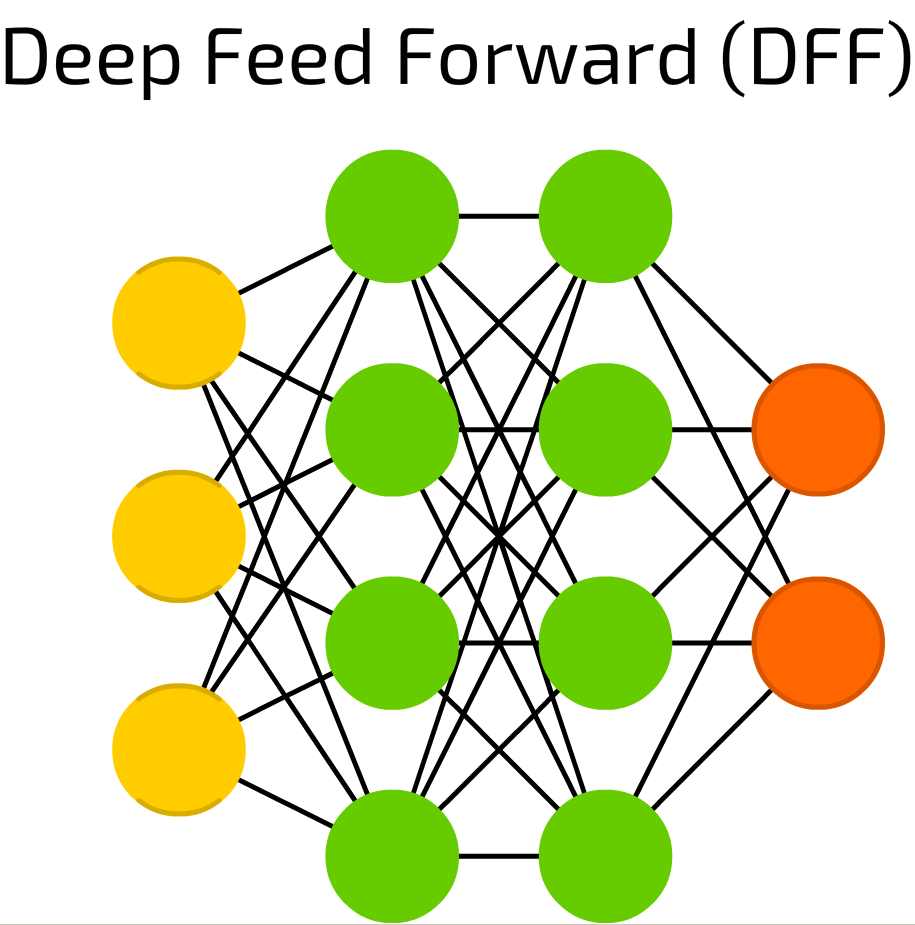
\includegraphics[scale=0.1]{model.png}
    \caption{Схема DFF сети}
    \label{fig:model}
\end{figure}

\section{Результаты}

В целом, неройнная сеть достаточно хорошо распознает котиков (например, она распознает котиков в профиль и в анфас, в прозрачных очках, и с незначительными перекрытиями морды). Однако, на некоторых порода собак, которые похожи на кошек, возможно ложное срабатывание. Так же, нейросеть не распознает нарисованных животных и кошек-сфинксов, что говорит о том, что кажется у "кошки" должна быть шерсть или ее подобие. В целом, такое качество работы нейронной сети обспечено за счет хороших датасетов. :wЖ

Пример работы программы

\texttt{input:}
\begin{figure}[h!]
    \centering
    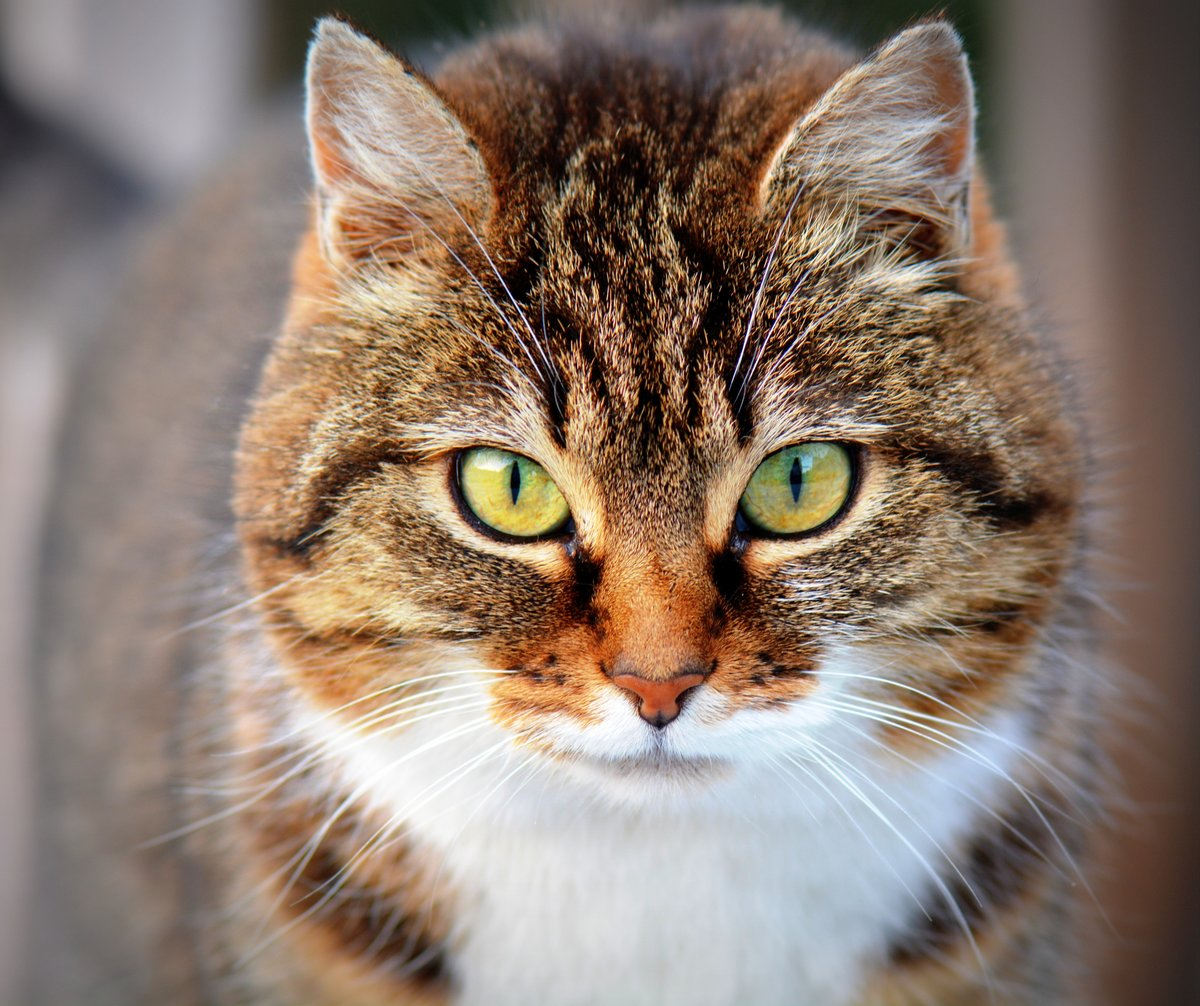
\includegraphics[scale=0.1]{input.png}
\end{figure}

\texttt{output: cat}


\begin{itemize}
    \item Код и подготовка данных - Данил Ельцов
    \item Анализ - Михаил Михайлов
    \item Отчет - Михаил Михайлов
\end{itemize}
\end{document}

